% This file was created with tikzplotlib v0.10.1.
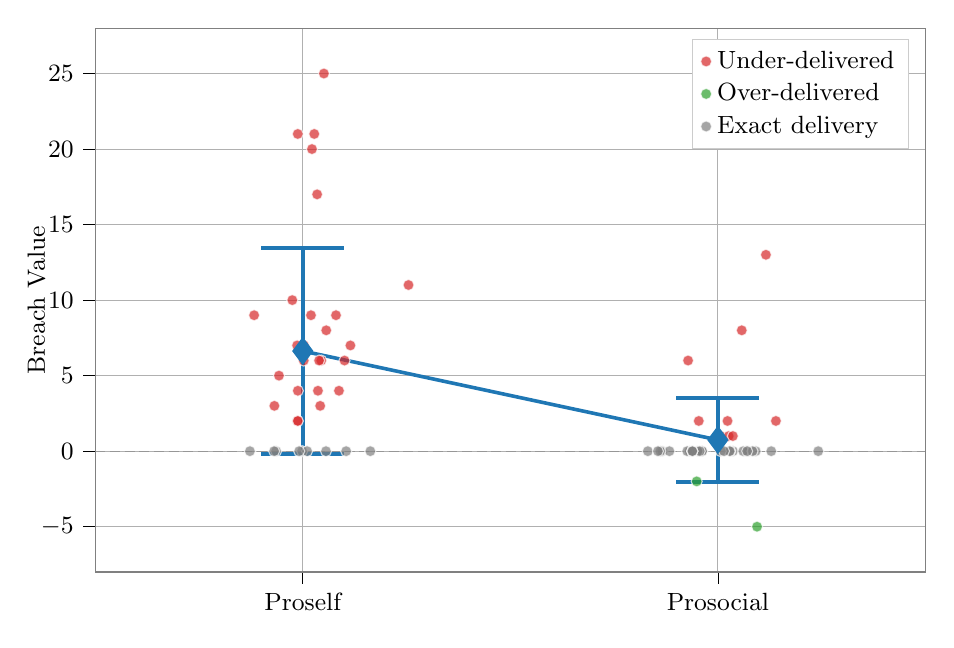
\begin{tikzpicture}[scale=1] % 整体缩放到原来的75%

\definecolor{crimson2143940}{RGB}{214,39,40}
\definecolor{darkgrey176}{RGB}{176,176,176}
\definecolor{forestgreen4416044}{RGB}{44,160,44}
\definecolor{grey}{RGB}{128,128,128}
\definecolor{grey127}{RGB}{127,127,127}
\definecolor{lightgrey204}{RGB}{204,204,204}
\definecolor{steelblue31119180}{RGB}{31,119,180}

\begin{axis}[
width=1\textwidth,    % 调整宽度
height=0.7\textwidth,   % 调整高度
axis line style={grey},
legend cell align={left},
legend style={
    fill opacity=1, 
    draw opacity=1, 
    text opacity=1, 
    draw=lightgrey204,
    font=\small        % 减小图例文字大小
},
tick align=outside,
tick pos=left,
tick label style={font=\small}, % 减小刻度标签文字大小
unbounded coords=jump,
x grid style={darkgrey176},
xmajorgrids,
xmin=-0.5, xmax=1.5,
xtick style={color=black},
xtick={0,1},
xticklabels={Proself,Prosocial},
y grid style={darkgrey176},
ylabel={Breach Value},
ylabel style={
    inner sep=0pt,    % 减少标签和轴的距离
    yshift=-5pt,
    font=\small% 微调标签位置
},
ymajorgrids,
ymin=-8, ymax=28,
ytick style={color=black}
]
\addplot [draw=white, fill=crimson2143940, mark=*, only marks, opacity=0.7]
table{%
x  y
0.0445638460840499 6
-0.0251492206481874 10
0.114781952236595 7
0.100617626838817 6
-0.0136131241983251 7
0.0872149291831909 4
-0.0572963889075815 5
-0.0118920383636059 4
-0.117137841801724 9
0.0509179870845854 25
0.0221982495680006 20
0.0346050065278643 17
0.00230769625747983 6
0.254731069003091 11
0.0393459215580669 6
-0.0120641631555385 21
0.0277365071623715 21
-0.0683417909118421 3
-0.0130147123380035 2
0.0420172585927707 3
-0.0118326818204489 2
0.0197717399460027 9
0.0800578994633806 9
0.0565739651290471 8
0.0365675958313638 4
0.00267953796925637 7
0.953947844949934 2
1.00659893512175 1
1.02599264664095 1
1.02320387746105 2
0.928213790904517 6
1.11573869264649 13
1.03610461954773 1
1.13981869672728 2
1.05748900969922 8
};
\addlegendentry{Under-delivered}
\addplot [draw=white, fill=forestgreen4416044, mark=*, only marks, opacity=0.7]
table{%
x  y
0.948996078943193 -2
1.09438747354748 -5
};
\addlegendentry{Over-delivered}
\addplot [draw=white, fill=grey127, mark=*, only marks, opacity=0.7]
table{%
x  y
-0.127308345407316 0
0.104520692071222 0
-0.0641762829563584 0
0.055957609290904 0
-0.0690108987612187 0
-0.00148865819560041 0
0.010467316369314 0
-0.00868031174757913 0
0.162803395945189 0
0.961671241805028 0
0.866342749234445 0
0.962145827755179 0
0.883295406035024 0
1.03623736893198 0
0.951216387630073 0
0.93821514743396 0
1.06768337023267 0
1.07418942436415 0
1.02972098441247 0
0.956204693829915 0
1.02844696233252 0
0.931802421814724 0
1.06119104521306 0
1.09106060861954 0
1.08352663180933 0
1.00699543775591 0
0.831289705831112 0
0.861294506495678 0
1.01475658604604 0
0.926218868506304 0
0.93826782575368 0
0.855588191755131 0
0.938356419492756 0
1.12858657125864 0
1.07049181342972 0
1.24179800517493 0
0.938632444210647 0
};
\addlegendentry{Exact delivery}
\addplot [line width=1.3pt, steelblue31119180, mark=diamond*, mark size=4.05, mark options={solid}, forget plot]
table {%
0 6.62857142857143
1 0.743589743589744
};
\addplot [line width=1.3pt, steelblue31119180, forget plot]
table {%
-0.1 -0.180098279475606
0.1 -0.180098279475606
nan nan
0 -0.180098279475606
0 13.4372411366185
nan nan
-0.1 13.4372411366185
0.1 13.4372411366185
};
\addplot [line width=1.3pt, steelblue31119180, forget plot]
table {%
0.9 -2.02577222661157
1.1 -2.02577222661157
nan nan
1 -2.02577222661157
1 3.51295171379106
nan nan
0.9 3.51295171379106
1.1 3.51295171379106
};
\addplot [grey, opacity=0.5, dash pattern=on 3.7pt off 1.6pt, forget plot]
table {%
-0.5 0
1.5 0
};
\end{axis}

\end{tikzpicture}